\section{Zeitdiskrete Zustandsraumdarstellung}

\subsection{Zeitdiskrete ZRD}{243-244}

Die Struktur der diskreten ZRD ist identisch wie die Struktur bei zeitkontinuierlichen Systemen.
Auch im diskreten Bereich kann eine UTF nicht eindeutig in eine ZRD übersetzt werden (Diagonalform, Beobachtungsnormalform, etc.).

\smallskip

\begin{minipage}[c]{0.63\columnwidth}
    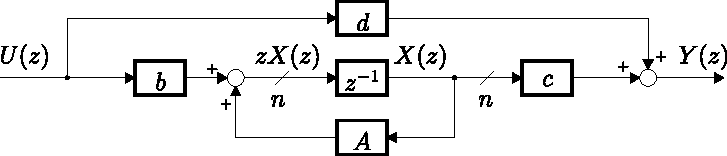
\includegraphics[width=\columnwidth, align=t]{images/diskrete_ZRD.pdf}
\end{minipage}
\hfill
\begin{minipage}[c]{0.35\columnwidth}
        \fbox{\parbox{0.9\columnwidth}{
            \vspace{-0.3cm}
            \begin{align*}
                x(k+1)  &= \bm{A} \cdot x(k) + b \cdot u(k) \\
                y(k)    &= b \cdot x(k) + d \cdot u(k)
            \end{align*}
            \vspace{-0.5cm}
    }}
\end{minipage}


\subsubsection{UTF aus diskreter ZRD}

\begin{minipage}[c]{0.44\columnwidth}
    Die diskrete UTF $G(z)$ kann jedoch eindeutig aus der ZRD bestimmt werden
\end{minipage}
\hfill
\begin{minipage}[c]{0.52\columnwidth}
    $$ G(z) = c \cdot (z \bm{I} - \bm{A})^{-1} \cdot b + d $$
\end{minipage}


\subsection{Stabilität}{245}

Das zeitdiskrete System ist \textbf{asymptotisch stabil}, wenn \textbf{alle Pole innerhalb des Einheitskreises liegen} (bzw. $\abs{z} < 1$ ist). \\
Unter Betrachtung der ZRD wird diese Bedingung interpretiert als:
Wenn alle \textbf{Eigenwerte} der \textbf{Systemmatrix} $\bm{A}$ (welche den Eigenwerten von $\bm{\Lambda} = \bm{A_{\rm Diag}}$ entsprechen)
einen \textbf{Betrag $< 1$} besitzen, ist das System \textbf{asymptotisch stabil}.

\vspace{-0.2cm}

$$ \boxed{ \det(\lambda \cdot \bm{I} - \bm{A}) \overset{!}{=} 0 \qquad \rightarrow \forall \lambda \quad  \abs{\lambda} < 1 \qquad \text{ \textrightarrow\ System asymptotisch stabil}}  $$

\textbf{Achtung: Umgekehrt gilt diese Aussage nicht!} Ein asymptotisch stabiles System bedeutet \textbf{nicht}, 
dass alle Eigenwerte der Systemmatrix $\bm{A}$ des Systems einen Betrag $< 1$ haben \textrightarrow\ Pol-/Nullstellenkürzungen


\subsection{Steuerbarkeit}{245}

\begin{outline}
    \1 Es gelten die (fast) äquivalenten Definitionen wie in zeitkontinuierlichen Systemen
    \1 Die Steuerbarkeit des Systems wird mit der Steuerbarkeitsmatrix bestimmt
\end{outline}


\subsubsection{Steuerbarkeitsmatrix $\bm{Q_S}$}

Ein System ist \textbf{vollständig steuerbar}, wenn
\begin{outline}
    \1 Der \textbf{Rang} der Steuerbarkeitsmatrix $\bm{Q_S}$ der Ordnung $n$ des Systems entspricht
        \2 Die Matrix $\bm{Q_S}$ hat somit vollen Rang
    \1 Bei Single-Input-System: ($m = 1$): Die \textbf{Determinante} von $\bm{Q_S}$ \textbf{ungleich Null ist}
\end{outline}

\vspace{-0.1cm}

$$
\boxed{ 
\bm{Q_S} = 
\begin{bmatrix}
    \bm{B} & \bm{A B} & \bm{A^2 B} & \cdots & \bm{A^{n-1} B} 
\end{bmatrix}
\qquad \qquad \text{ Dimension: } n \times (n \cdot m)
}
$$

\begin{minipage}[c]{0.48\columnwidth}
    \begin{tabular}{ll}
        $\bm{A}$    & Systemmatrix ($n \times n$)   \\
        $\bm{B}$    & Eingangsmatrix ($n \times m$) \\
    \end{tabular}
\end{minipage}
\hfill
\begin{minipage}[c]{0.48\columnwidth}
    \begin{tabular}{ll}
        $n$         & Zustände \\
        $m$         & Eingänge \\
    \end{tabular}
\end{minipage}


\subsection{Beobachtbarkeit}{245}

\begin{outline}
    \1 Es gelten die (fast) äquivalenten Definitionen wie in zeitkontinuierlichen Systemen
    \1 Die Beobachtbarkeit des Systems wird mit der Beobachtbarkeitsmatrix bestimmt
\end{outline}


\subsubsection{Beobachtbarkeitsmatrix $\bm{Q_B}$}

Ein System ist \textbf{vollständig beobachtbar}, wenn

\begin{outline}
    \1 Der \textbf{Rang} der Beobachtbarkeitsmatrix $\bm{Q_B}$ der Ordnung $n$ des Systems entspricht
        \2 Die Matrix $\bm{Q_B}$ hat somit vollen Rang
    \1 Bei Single-Output-System:  Die \textbf{Determinante} von $\bm{Q_B}$ \textbf{ungleich Null ist}
\end{outline}

\smallskip

\begin{minipage}[c]{0.4\columnwidth}
    $$
    \bm{Q}_B = 
    \begin{bmatrix}
        \bm{C} \\ \bm{C A} \\ \bm{C A^2} \\ \vdots \\ \bm{C A^{n-1}} 
    \end{bmatrix}
    $$
\end{minipage}
\hfill
\begin{minipage}[c]{0.58\columnwidth}
    \begin{tabular}{ll}
        Dimension:  & $(k \cdot n) \times n$ \\
        $\bm{A}$    & Systemmatrix ($n \times n$) \\
        $\bm{C}$    & Beobachtungsmatrix ($k \times m$) \\
        $n$         & Zustände \\
        $m$         & Eingänge \\
        $k$         & Ausgänge 
    \end{tabular}
\end{minipage}


\columnbreak

